\scanpage{7}
\mspage{\textcircled{3}}

% The upper calculations are canceled en bloc by three long oblique strokes
% and a sweeping left/bottom boundary. Each complete diagram, including its
% arrow paths, is wrapped in deleted; mbox keeps its drawing indivisible.
\[
\deleted{p_0p_{12}=p_0p_{13}=p_0\underset{p_{31}}{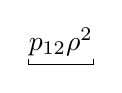
\begin{tikzpicture}[baseline=(t.base)]\node[inner sep=0pt](t){$p_{12}\rho^2$};\draw ([yshift=-1pt]t.south west)--([yshift=-3pt]t.south west)--([yshift=-3pt]t.south east)--([yshift=-1pt]t.south east);\end{tikzpicture}}\sigma_2}
\qquad
\deleted{\rho^2\sigma_2=\sigma_3\rho^2}
\]
\diagram{\deleted{\mbox{\begin{tikzpicture}[x=1cm,y=1cm]
\node at (0,0) {$(x,y,z)$};
\node at (3.6,0) {$(z,y,x)$};
\draw (1.15,-0.12)--(1.15,0.12);
\draw[->] (1.15,0)--(2.30,0);
\draw (2.30,0.14)--(2.50,0)--(2.30,-0.14);
\draw[->] (1.15,-0.8)--(2.50,-0.8);
\node at (3.6,-0.8) {$(x,z)$};
\draw[->] (4.5,-0.8)--(5.4,-0.8);
\node at (5.8,-0.8) {$x$};
\end{tikzpicture}}}}
\[\deleted{p_0p_{12}\sigma_1=p_0p_{12}}\]
\[\deleted{(\unsure{x},\unsure{x|z},y)}\]
% The continuation shaft has a separate tail bar and a small loop at its
% right endpoint. It is not replaced by the clear chevron of the row above.
\diagram{\deleted{\mbox{\begin{tikzpicture}[x=1cm,y=1cm]
\node[anchor=east] at (-0.8,0) {$\rho^2\sigma_2:$};
\node at (0.45,0) {$(x,y,z)$};
\node at (3.8,0) {$(z,y,x))$};
\draw[|->] (1.65,0)--(2.6,0);
\draw (0.96,-0.89)--(0.96,-0.65);
\draw (1.1,-0.78)--(2.6,-0.69);
\draw (2.6,-0.79)--(2.6,-0.62)
  .. controls (2.64,-0.53) and (2.78,-0.59) .. (2.7,-0.65)
  --(2.6,-0.69);
\node at (3.8,-0.78) {$(\begin{tikzpicture}[baseline=(t.base)]\node[inner sep=0pt](t){$y,x$};\draw ([yshift=-1pt]t.south west)--([yshift=-3pt]t.south west)--([yshift=-3pt]t.south east)--([yshift=-1pt]t.south east);\end{tikzpicture},z)$};
\end{tikzpicture}}}}
\[
\begin{array}{ll}
\deleted{\delta_1\sigma=(x\unsure{,}y,y)}&{}\\[0.7ex]
\deleted{(x,\unsure{x|z},y)}&\qquad\deleted{z,x,y}\\[0.7ex]
\deleted{(y,y,x)}&{}
\end{array}
\]
% Tail bar and square downturned terminal are both visible; no chevron
% is supplied to the last coordinate mapping.
\diagram{\deleted{\mbox{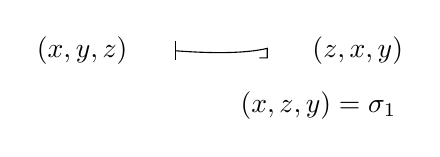
\begin{tikzpicture}[x=1cm,y=1cm]
\node at (0,0) {$(x,y,z)$};
\node at (3.5,0) {$(z,x,y)$};
\draw (1.18,-0.12)--(1.18,0.12);
\draw (1.18,0) .. controls (1.7,-0.04) and (2.1,-0.03) .. (2.35,0.03)
  --(2.35,-0.09)--(2.25,-0.09);
\node at (3.0,-0.7) {$(x,z,y)=\sigma_1$};
\end{tikzpicture}}}}

\mspage{\textcircled{3}}
Si $E_0$ est réduit à un p\textsuperscript{t}, donc par $\delta_0,\delta_1\delta_0$ $E_1,E_2$ deviennent des ens. pointés, et $\mathcal G_2,\mathcal G_3$ respectent la ponctuation.
\margin{(``ponctués'')}
\deleted{\unsure{Donc.|On a.}}
$\deleted{\delta_1}$ \deleted{respecte \unsure{les|le}}
Donc, en plus des opérations de $\mathcal G_2,\mathcal G_3$, on a
\diagram{\begin{tikzcd}[ampersand replacement=\&,column sep=large]
E_1\arrow[r,bend right=35,"\delta_1"']\&E_2\arrow[l,"p_{12}"']
\end{tikzcd}}
, où $\delta_1$ \inserted{et $p_{12}$} respect\unsure{ent}%
% The terminal low loop, high arch and return touch the right paper edge;
% the compressed n/t cannot be separated securely. No punctuation supplied.
\ les ponctuations, et où $p_{12},\delta_1$ satisfont aux cinq relations supplémentaires
\diagram{\begin{tikzpicture}[x=0.8cm,y=0.8cm,every node/.style={font=\footnotesize,inner sep=1pt}]
% Open pen joins at upper left and bottom left; right upright overruns bottom.
\draw (0.18,0)--(20,0.40)--(20,-6.25);
\draw (0,-0.38)--(0.22,-5.98);
\draw (0.37,-5.98)--(20,-5.78);
% Inner compartment uses the outer right and bottom borders.
\draw[->] (9.95,-2.30)--(20,-1.96);
\draw (9.86,-2.65)--(10.05,-6.05);
\node[anchor=west] at (0.45,-0.55) {$p_{12}\delta_1=\sigma$};
\node[anchor=west] at (0.45,-1.65) {$p_{12}\underset{\delta_3}{\begin{tikzpicture}[baseline=(t.base)]\node[inner sep=0pt](t){$\rho\delta_1$};\draw ([yshift=-1pt]t.south west)--([yshift=-3pt]t.south west)--([yshift=-3pt]t.south east)--([yshift=-1pt]t.south east);\end{tikzpicture}}=\text{application constante de valeur }e_1\quad\text{(p\textsuperscript{t} marqué de }E_1\text{)}$};
\node[anchor=west] at (0.45,-3.05) {$p_{12}\underset{\delta_2}{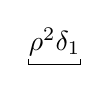
\begin{tikzpicture}[baseline=(t.base)]\node[inner sep=0pt](t){$\rho^2\delta_1$};\draw ([yshift=-1pt]t.south west)--([yshift=-3pt]t.south west)--([yshift=-3pt]t.south east)--([yshift=-1pt]t.south east);\end{tikzpicture}}=\mathrm{id}_{E_1}$};
\node[anchor=west] at (0.45,-4.35) {$\sigma_1\delta_1=\delta_1$};
\node[anchor=west] at (0.45,-5.45) {$p_{12}\sigma_3=\sigma p_{12}$};
\node[anchor=west] at (10.1,-2.95) {$p_{12}\delta_2=\mathrm{id}_{E_1}$};
\node[anchor=west] at (10.1,-4.05) {$p_{12}\underset{\delta_1}{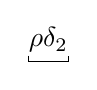
\begin{tikzpicture}[baseline=(t.base)]\node[inner sep=0pt](t){$\rho\delta_2$};\draw ([yshift=-1pt]t.south west)--([yshift=-3pt]t.south west)--([yshift=-3pt]t.south east)--([yshift=-1pt]t.south east);\end{tikzpicture}}=\sigma$};
\node[anchor=west] at (10.1,-5.25) {$p_{12}\underset{\delta_3}{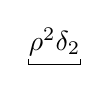
\begin{tikzpicture}[baseline=(t.base)]\node[inner sep=0pt](t){$\rho^2\delta_2$};\draw ([yshift=-1pt]t.south west)--([yshift=-3pt]t.south west)--([yshift=-3pt]t.south east)--([yshift=-1pt]t.south east);\end{tikzpicture}}=e_1$};
\node[anchor=north west,font=\tiny] at (14.0,-4.90) {$\begin{gathered}\text{(\unsure{application|\deleted{appl} constante}}\\\text{de }E_1\text{ sur}\\e_{\unsure{1|q}}\text{)}\end{gathered}$};
\node[anchor=west] at (15.55,-2.45) {$\uline{p_{12}\sigma_3=\sigma p_{11}}$};
\node[anchor=west] at (16.05,-3.10) {$\sigma_2\delta_2=\delta_2$};
\node[anchor=west] at (16.65,-3.95) {$\deleted{p_{\unsure{12}}\sigma_3\unsure{=\sigma}p_{12}}$};
\node[anchor=west] at (16.25,-4.65) {$\deleted{\unsure{\mathrm{id}}}$};
% The oblique line is part of the crossing of the two canceled entries.
\draw[line width=0.9pt] (15.65,-2.85)--(18.15,-5.0);
\node at (18.7,-5.05) {$E_1$};
\node at (21.6,-5.05) {$E_2$};
\draw[->] (21.0,-5.05)--(19.25,-5.05);
\node at (20.1,-4.72) {$p_{12}$};
\draw[->] (19.25,-5.43) .. controls (19.8,-5.60) and (20.55,-5.60) .. (21.0,-5.43);
\node at (20.1,-5.85) {$\delta_1$};
\end{tikzpicture}}
\margin{6}
